\documentclass{beamer}
\usepackage{array}
\usepackage{graphicx}
\usepackage{xcolor}
\usepackage{graphicx}
\usepackage{amsmath}

\usetheme{Madrid}

% Suppress the navigation bar and remove name and date from slides
\setbeamertemplate{navigation symbols}{}
\setbeamertemplate{footline}{}  % Removes the footer line with the author and date
\setbeamertemplate{headline}{}  % Removes the header line

% Title page details
\title{Conversational Used Car Price Predictor}
\subtitle{CS702 - Computing Lab}
\author{ABHIJITH C \and ANAND M K}
\institute{Department of Computer Science and Engineering \\ NITK Surathkal}
\date{}  % No date on title slide

\begin{document}

% Title page
\begin{frame}[t]
    \titlepage
\end{frame}

\begin{frame}[t]{Introduction}
    \begin{itemize}
        \item This project focuses on developing a \textbf{Conversational Used Car Price Predictor}, integrating a chatbot interface with a machine learning model.
        \item \textbf{Goal:} To allow users to interact through natural conversation rather than filling out traditional forms to predict used car prices.
        \item The chatbot will collect necessary car details (brand, model, year, mileage, etc.) step by step through an intuitive and engaging interface.
        \item A machine learning model will use the gathered data to predict the price of the used car, ensuring accurate and reliable predictions.
        \item The chatbot also handles additional queries, such as explaining how the price was calculated or what factors affect the car’s value.
    \end{itemize}
\end{frame}


\begin{frame}{System Architecture}'
    \centering
   	 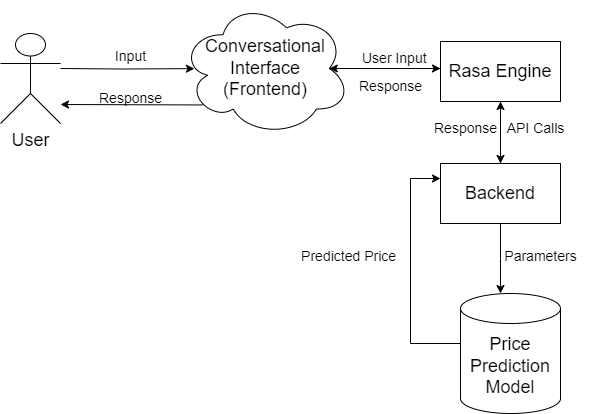
\includegraphics[width=0.8\textwidth]{Midsem.drawio.png}
\end{frame}


\begin{frame}{Project Overview: Progress and Next Steps}
    \begin{itemize}
        \item \textbf{Milestones Achieved:}
        \begin{itemize}
            \item Data collection and preprocessing for the car price prediction model.
            \item Model development using \textbf{Random Forest} and SHAP calculation for feature contribution analysis.
            \item Integration of the backend with Rasa.
            \item Development of a sample chatbot to collect car parameters from the user.
            \item Validation of user input parameters in the Rasa chatbot.
        \end{itemize}
        
        \item \textbf{\textcolor{gray}{Upcoming Work:}}
        \begin{itemize}
            \item \textcolor{gray}{Improve the Rasa chatbot by adding more test data.}
            \item \textcolor{gray}{Handle general questions in Rasa.}
        \end{itemize}
    \end{itemize}
\end{frame}

\begin{frame}{Backend API Creation}
    \begin{itemize}
        \item \textbf{Framework Used:} Flask
        \begin{itemize}
            \item A lightweight web framework for Python, used to create web applications.
        \end{itemize}
        
        \item \textbf{Endpoints:}
        \begin{itemize}
            \item \texttt{/predict\_price}: 
            \begin{itemize}
                \item Accepts car attributes as query parameters.
                \item Returns the predicted selling price of the car.
            \end{itemize}
            \item \texttt{/max\_contribution}: 
            \begin{itemize}
                \item Accepts the same car attributes as query parameters.
                \item Returns the highest contributing feature to the predicted price and its percentage contribution.
            \end{itemize}
        \end{itemize}
        
        \item \textbf{Input Handling:}
        \begin{itemize}
            \item Retrieves input data via query parameters (GET API).
        \end{itemize}
        
        \item \textbf{Response Format:}
        \begin{itemize}
            \item Outputs predictions and contributions as JSON, facilitating easy integration with frontend applications.
        \end{itemize}
    \end{itemize}
\end{frame}

\begin{frame}
	\frametitle{Intents in NLU}
	
	\begin{itemize}
		\item \textbf{greet} - Intent for greetings
		\item \textbf{goodbye} - Intent for farewells
		\item \textbf{affirm} - Intent for confirming or agreeing
		\item \textbf{deny} - Intent for negating or disagreeing
		\item \textbf{bot\_challenge} - Intent for asking about the nature of the bot
		\item \textbf{inform} - Intent for providing car details like brand, model, mileage, etc.
		\item \textbf{stop} - Intent to stop the conversation
		\item \textbf{ask\_shap} - Intent to ask about factors impacting price
	\end{itemize}
	
\end{frame}


\begin{frame}
	\frametitle{Entities in NLU}
	
	\begin{itemize}
		\item \textbf{brand} - represents the car brand (e.g., Toyota, Ford, etc.)
		\item \textbf{model} - represents the car model (e.g., Fortuner, Swift, etc.)
		\item \textbf{mileage} - represents the car's mileage (e.g., 15 km/l)
		\item \textbf{km\_driven} - represents the distance the car has been driven (e.g., 10000 km)
		\item \textbf{fuel\_type} - represents the type of fuel the car uses (e.g., petrol, diesel)
		\item \textbf{transmission\_type} - represents the transmission type of the car (e.g., manual, automatic)
		\item \textbf{engine} - represents the engine capacity of the car (e.g., 1500 cc)
		\item \textbf{max\_power} - represents the car's maximum power (e.g., 150 bhp)
		\item \textbf{seats} - represents the seating capacity of the car (e.g., 5 seats)
		\item \textbf{year\_of\_manufacture} - represents the car's year of manufacture (e.g., 2020)
	\end{itemize}
	
\end{frame}

	
\begin{frame}{Entity Extraction using Regex and Lookup Tables}
	
	\begin{itemize}
		\item \textbf{Regex Patterns for Entity Extraction:}
		\begin{itemize}
			\item \textbf{km\_driven}
			\item \textbf{mileage} 
			\item \textbf{engine} 
			\item \textbf{max\_power} 
			\item \textbf{seats} 
			\item \textbf{year\_of\_manufacture}
			\item \texttt{Example:\textbackslash b\d\{1,2\}\textbackslash b(?=\textbackslash s\*(kmpl\textbar km\textbackslash l\textbar km\ per\ liter)\textbackslash b)\newline} 
			15 kmpl, 18 km/l
		\end{itemize}
		
		\item \textbf{Lookup Tables for Entity Extraction:}
		\begin{itemize}
			\item \textbf{brand}: Maruti, Hyundai, Ford, Renault, Mini, Mercedes-Benz, etc.
			\item \textbf{model}: Alto, Grand, i20, Ecosport, Wagon R, i10, Venue, Swift, etc.
			\item \textbf{transmission\_type}: manual, automatic
			\item \textbf{fuel\_type}: petrol, diesel, electric
		\end{itemize}
	\end{itemize}
	
\end{frame}


\begin{frame}{Form: \texttt{car\_details\_form}}
	\begin{itemize}
		\item The form defines set of required slots that need to be filled.
		\item When form is active, the system will ask the user for details (one by one), and as the user provides answers, the values will populate the respective slots.
		\item Form deactivates after all slots are filled.
		\item \textbf{Required Slots}:
		\begin{itemize}
			\item \texttt{brand}, \texttt{model}, \texttt{km\_driven}, \texttt{mileage}, \texttt{fuel\_type}, 
			\item \texttt{transmission\_type}, \texttt{engine}, \texttt{max\_power}, \texttt{seats}, \texttt{year\_of\_manufacture}
		\end{itemize}
		\item \textbf{Slot Mappings}:
		\begin{itemize}
			\item Each slot corresponds to an entity, e.g., \texttt{brand} is mapped to the \texttt{brand} entity.
			\item These mappings allow automatic extraction from user input.
		\end{itemize}
	\end{itemize}
\end{frame}

\begin{frame}{Actions}
	\begin{itemize}
		\item \textbf{utter\_slots\_values}: Confirms the filled slot values.
		\item \textbf{utter\_greet}: Greets the user and starts the conversation.
		\item \textbf{utter\_goodbye}: Ends the conversation.
		\item \textbf{utter\_iamabot}: Informs the user that the assistant is a virtual bot.
		\item \textbf{utter\_ask\_brand}, \textbf{utter\_ask\_model}, \dots : Asks the user for specific slot values like brand, model, mileage, etc.
		\item \textbf{action\_clear\_slots}: Clears the filled slots.
		\item \textbf{action\_predict\_car\_price}: Triggers the car price prediction.
		\item \textbf{utter\_please\_rephrase}: Asks the user to rephrase if the input is unclear.
		\item \textbf{action\_max\_contribution}: Returns the feature with the highest contribution to the price prediction.
		\item \textbf{validate\_car\_details\_form}: Validates filled slots to ensure correct information.
	\end{itemize}
\end{frame}

\begin{frame}{ValidateCarDetailsForm - Slot Validation}
	\begin{itemize}
		\item \textbf{Brand \& Model}: Fuzzy matching with predefined lists of car brands/models.
		\item \textbf{Numeric Slots}: Checks ranges for km driven, mileage, engine capacity, max power, seats, and year of manufacture.
		\item \textbf{Fuel Type \& Transmission}: Validates against allowed values like \texttt{petrol}, \texttt{diesel}, \texttt{automatic}, etc.
	\end{itemize}
\end{frame}

\begin{frame}{Telegram Integration}
	
	\begin{itemize}
		\item Rasa provides an API endpoint (default: \texttt{http://localhost:5005/webhooks/telegram/webhook}) to handle incoming messages.
		\item The endpoint allows Rasa to receive and send messages to Telegram through webhooks.
		\item Telegram bot integration:
		\begin{itemize}
			\item Create a bot using \texttt{BotFather} on Telegram and obtain a token.
			\item Set the Telegram bot token in Rasa configuration \texttt{credentials.yml}.
		\end{itemize}
		\item Rasa listens to messages from users on Telegram, processes them, and sends back responses via the webhook.
	\end{itemize}
	
\end{frame}

\begin{frame}{Upcoming Work}
    \begin{itemize}
        \item Improve the Rasa chatbot by adding more test data to enhance its understanding and responsiveness.
        \item Handle general questions within the chatbot to improve user engagement and satisfaction.
    \end{itemize}
\end{frame}


\begin{frame}[t]{References}
\begin{thebibliography}{9}

\bibitem{rasa}
Rasa Technologies, ``Rasa Documentation,'' \textit{Rasa}, 2023. [Online]. Available: \texttt{https://rasa.com/docs/}
\bibitem{flask}
Armin Ronacher, ``Flask Documentation,'' \textit{Flask}, 2023. [Online]. Available: \texttt{https://flask.palletsprojects.com/}


\bibitem{shap-doc}
SHAP Documentation, ``SHAP (SHapley Additive exPlanations),'' 2023. [Online]. Available: \texttt{https://shap.readthedocs.io/en/latest/}

\bibitem{randomforest}
Leo Breiman, ``Random Forests,'' \textit{Machine Learning}, vol. 45, no. 1, 2001, pp. 5-32. [Online]. Available: \texttt{https://link.springer.com/article/10.1023/A:1010933404324}

\bibitem{randomforest-doc}
Scikit-learn, ``Random Forests,'' 2023. [Online]. Available: \texttt{https://scikit-learn.org/dev/modules/generated/\\sklearn.ensemble.RandomForestRegressor.html}



\end{thebibliography}
\end{frame}



\begin{frame}[t]{.}
    \centering
    \vspace{1cm}
    \textbf{\Huge{}}
    
    \vspace{0.5cm}
    \rule{0.5\textwidth}{0.5mm} % Horizontal line for design

    \vspace{1cm}
    \textbf{\Large{Thank You!}}

    \vspace{0.5cm}
    \rule{0.5\textwidth}{0.5mm} % Another horizontal line for symmetry
\end{frame}


\end{document}
